\subsection{Semantic Disentanglement-based Methods}

\textit{\textbf{FREE}: Feature Refinement for Generalized Zero-Shot Learning}~\cite{Chen2021FREE} (2021) use a feature refinement module to jointly map the semantic and visual modalities, and refine the visual features of seen and unseen class samples -- dropping unnecessary information from the visual features. They use the class label supervision and a semantic cycle-consistency
constraint to guide the proposed module to learn relevant feature representations that are also semantically relevant with respect to their corresponding classes.


\textit{Semantics Disentangling for Generalized Zero-Shot Learning (\textbf{SDGZSL})}~\cite{SDGZSL} (2021) introduce a total correlation penalty that is applied to the visual features of unseen classes that were generated by a conditional VAE~\cite{VAEs}. This work uses a Relation Network~\cite{RelNetwork} to correlate the factorized estimated features -- the \textit{semantic-consistent} and the \textit{semantic-unrelated} latent features.


\begin{figure*}[tp]
\begin{minipage}[t]{0.32\textwidth}
  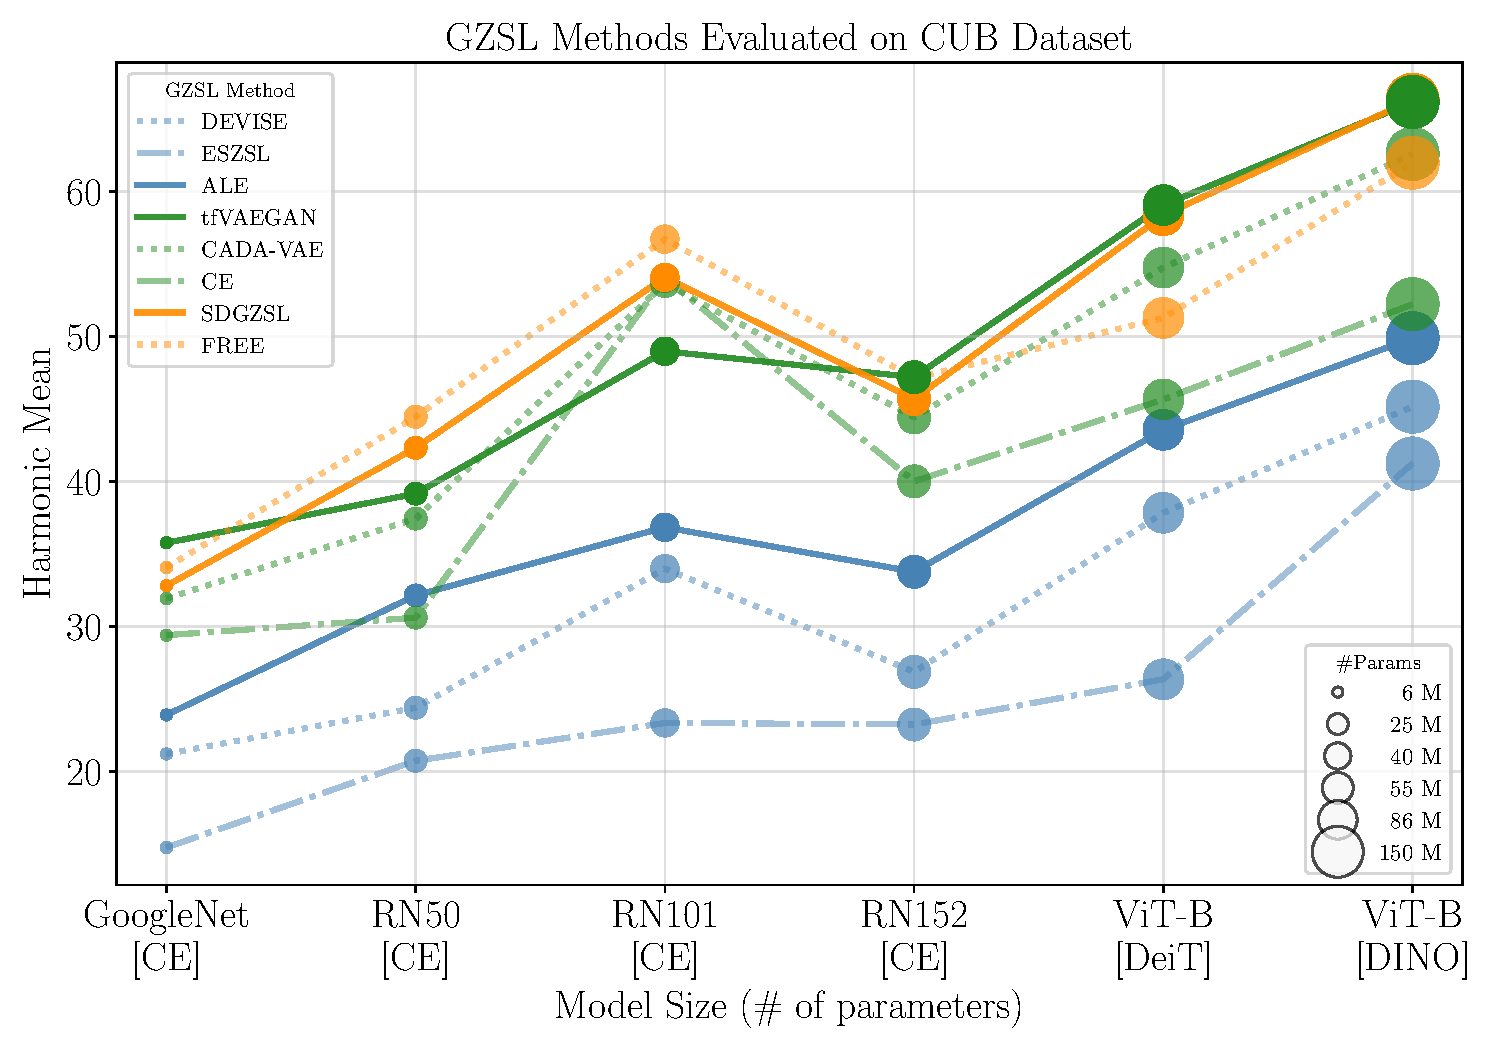
\includegraphics[align=t,width=\linewidth]{Images/cub_noclip_noft.pdf}
\end{minipage}%
\hfill % maximize the horizontal separation
\begin{minipage}[t]{0.32\textwidth}
  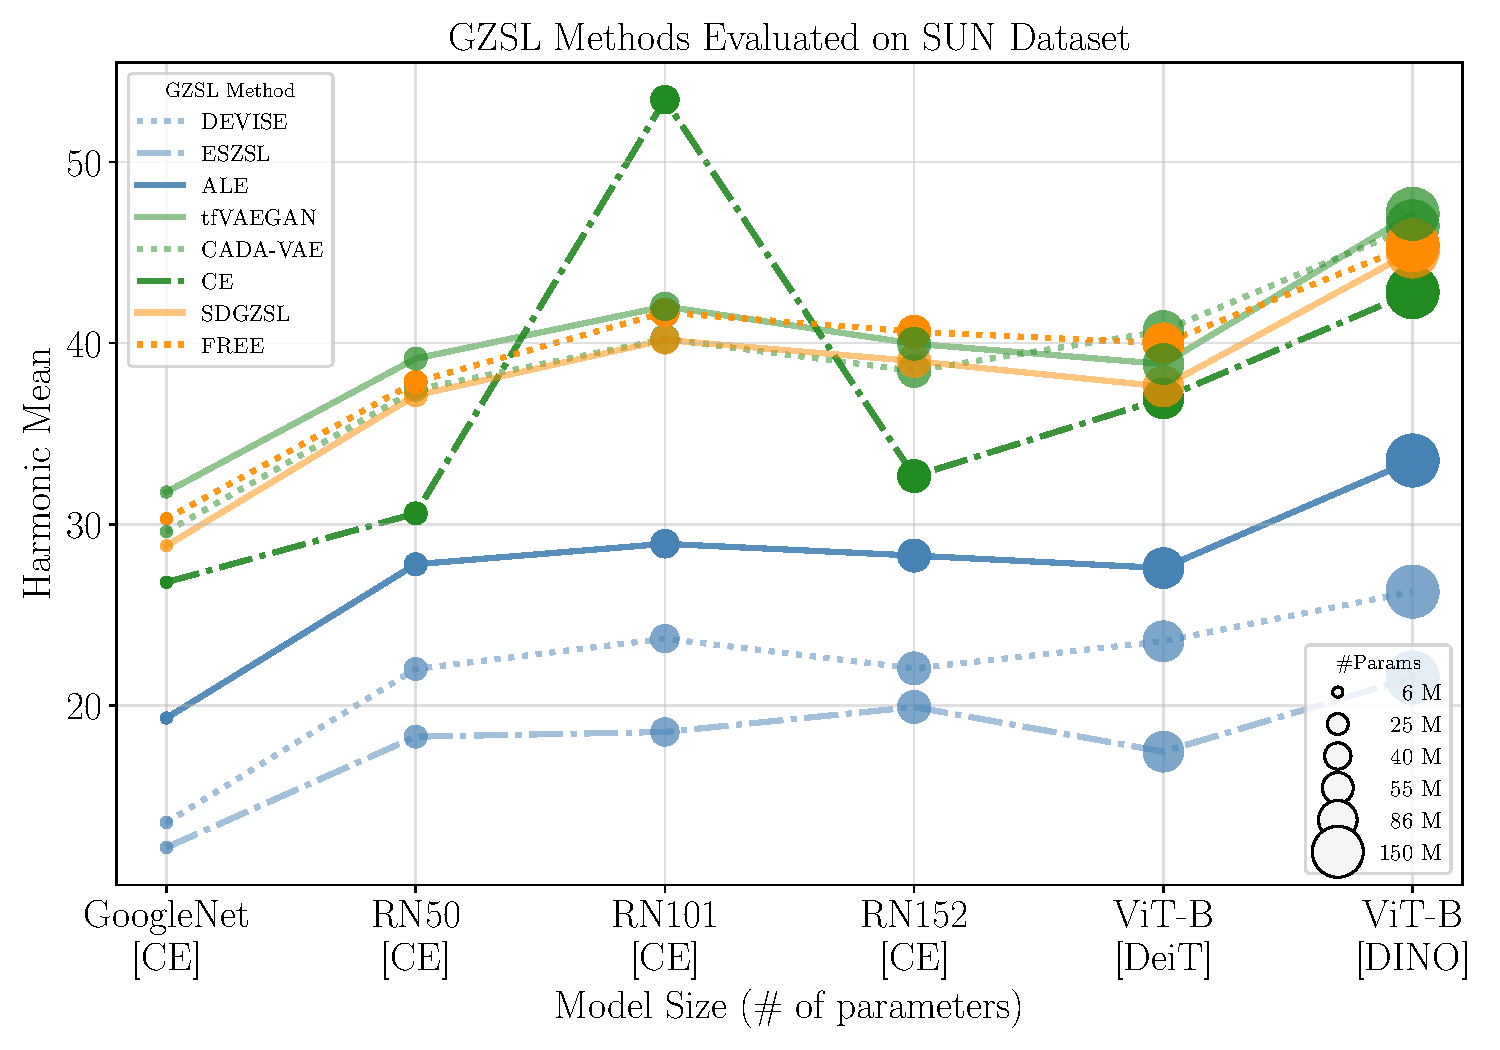
\includegraphics[align=t,width=\linewidth]{Images/sun_noclip_noft.pdf}
\end{minipage}%
\hfill
\begin{minipage}[t]{0.35\textwidth}
  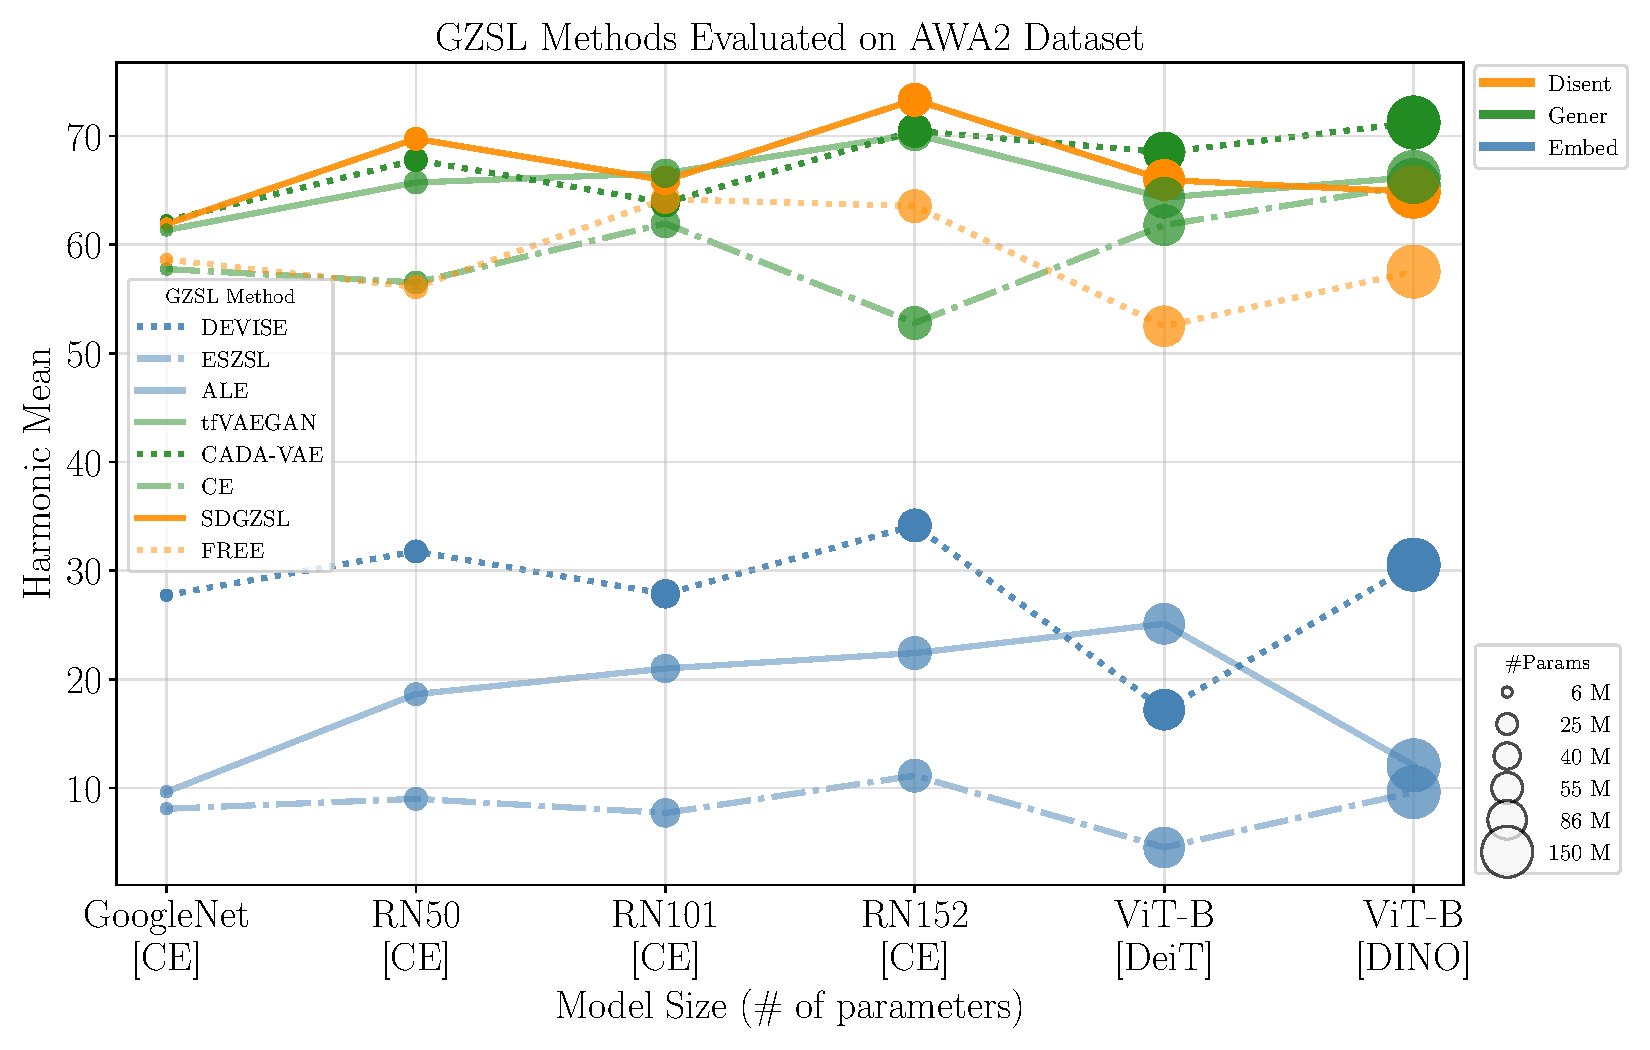
\includegraphics[align=t,width=\linewidth]{Images/awa2_noclip_noft.pdf}
\end{minipage}%
 % \vspace{-0.05in}
 \caption{\textbf{Impact of Model Parameter Size.} We show the Harmonic Mean performance of different methods when using a specific model to extract the features of image samples from CUB, SUN, and AWA2 datasets. All models were pre-trained using ImageNet-1k. The blue lines correspond to the embedding-based methods, the green lines correspond to the generative-based methods, and the orange lines correspond to the semantic disentanglement-based methods. Best viewed in color.}
 \label{fig:model_backbone_size_vs_method}
\end{figure*}


\begin{figure*}[bp]
\begin{minipage}[t]{0.33\textwidth}
  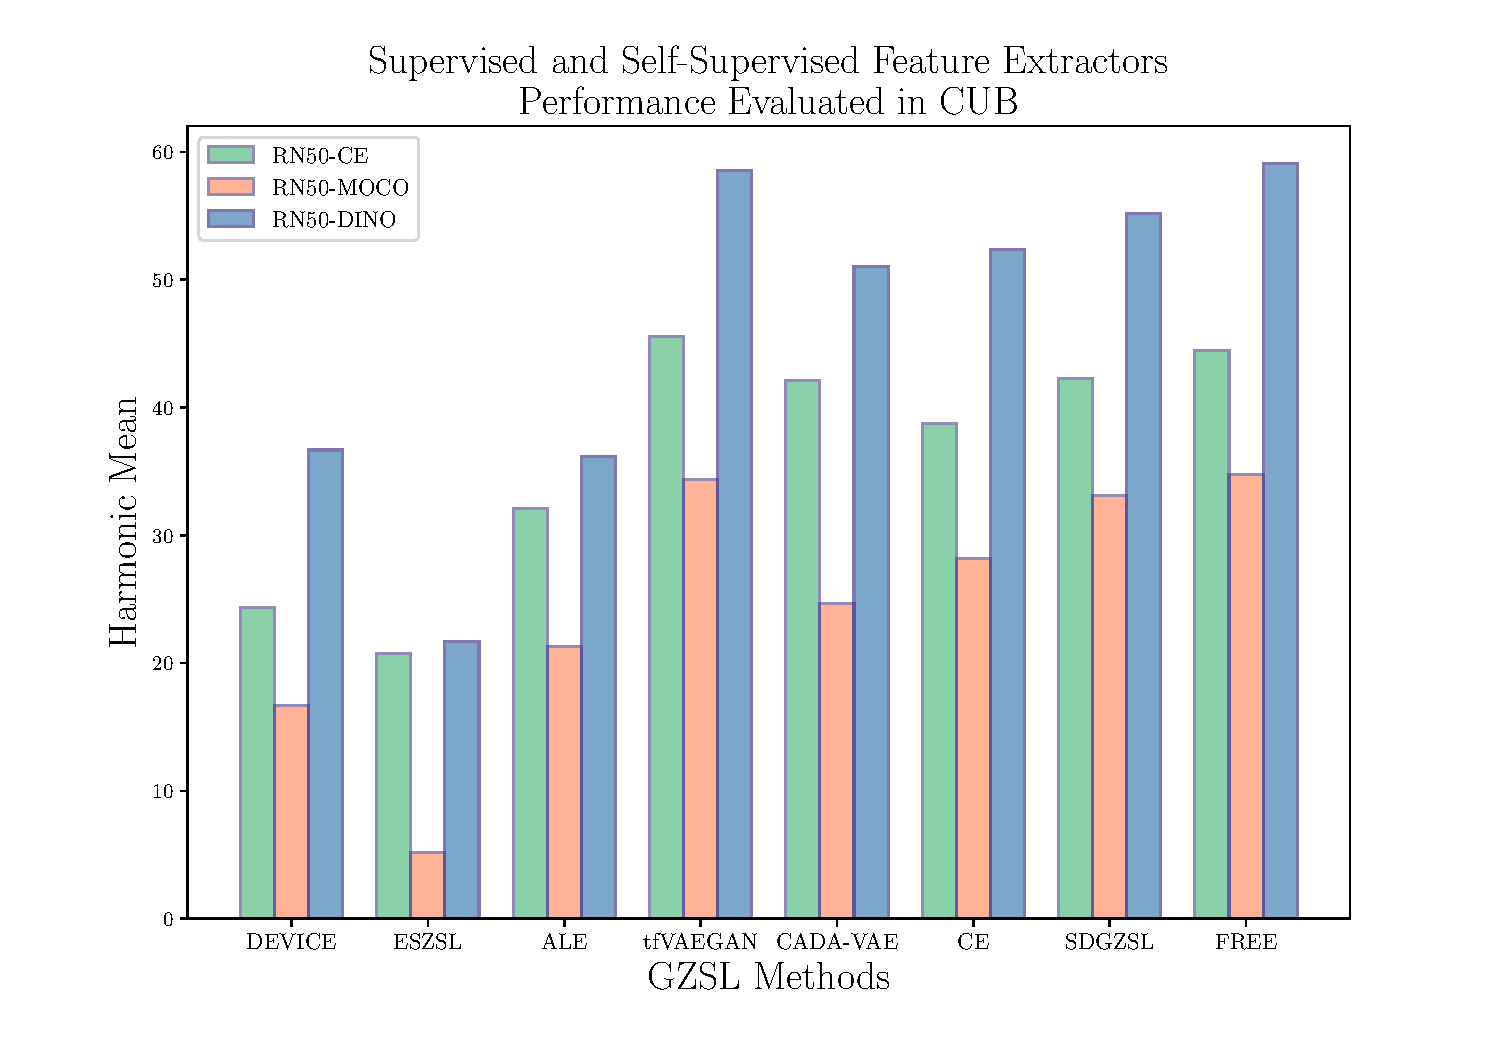
\includegraphics[align=t,width=\linewidth]{Images/cub_diff_objs.pdf}
\end{minipage}%
\hfill % maximize the horizontal separation
\begin{minipage}[t]{0.33\textwidth}
  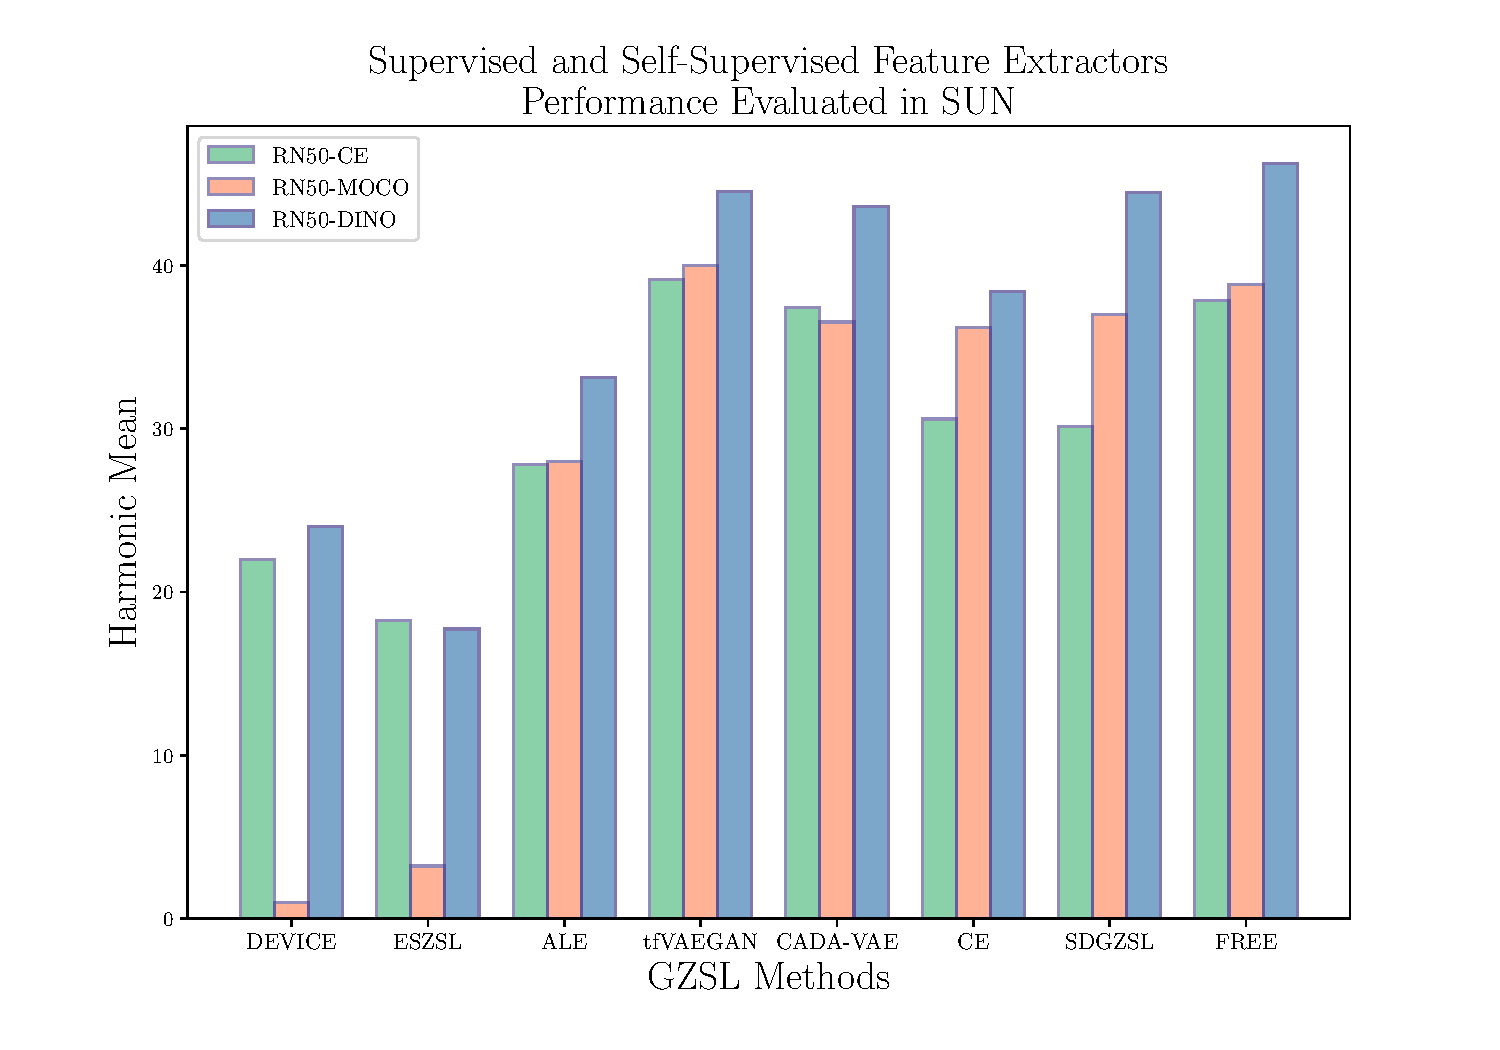
\includegraphics[align=t,width=\linewidth]{Images/sun_diff_objs.pdf}
\end{minipage}%
\hfill
\begin{minipage}[t]{0.33\textwidth}
  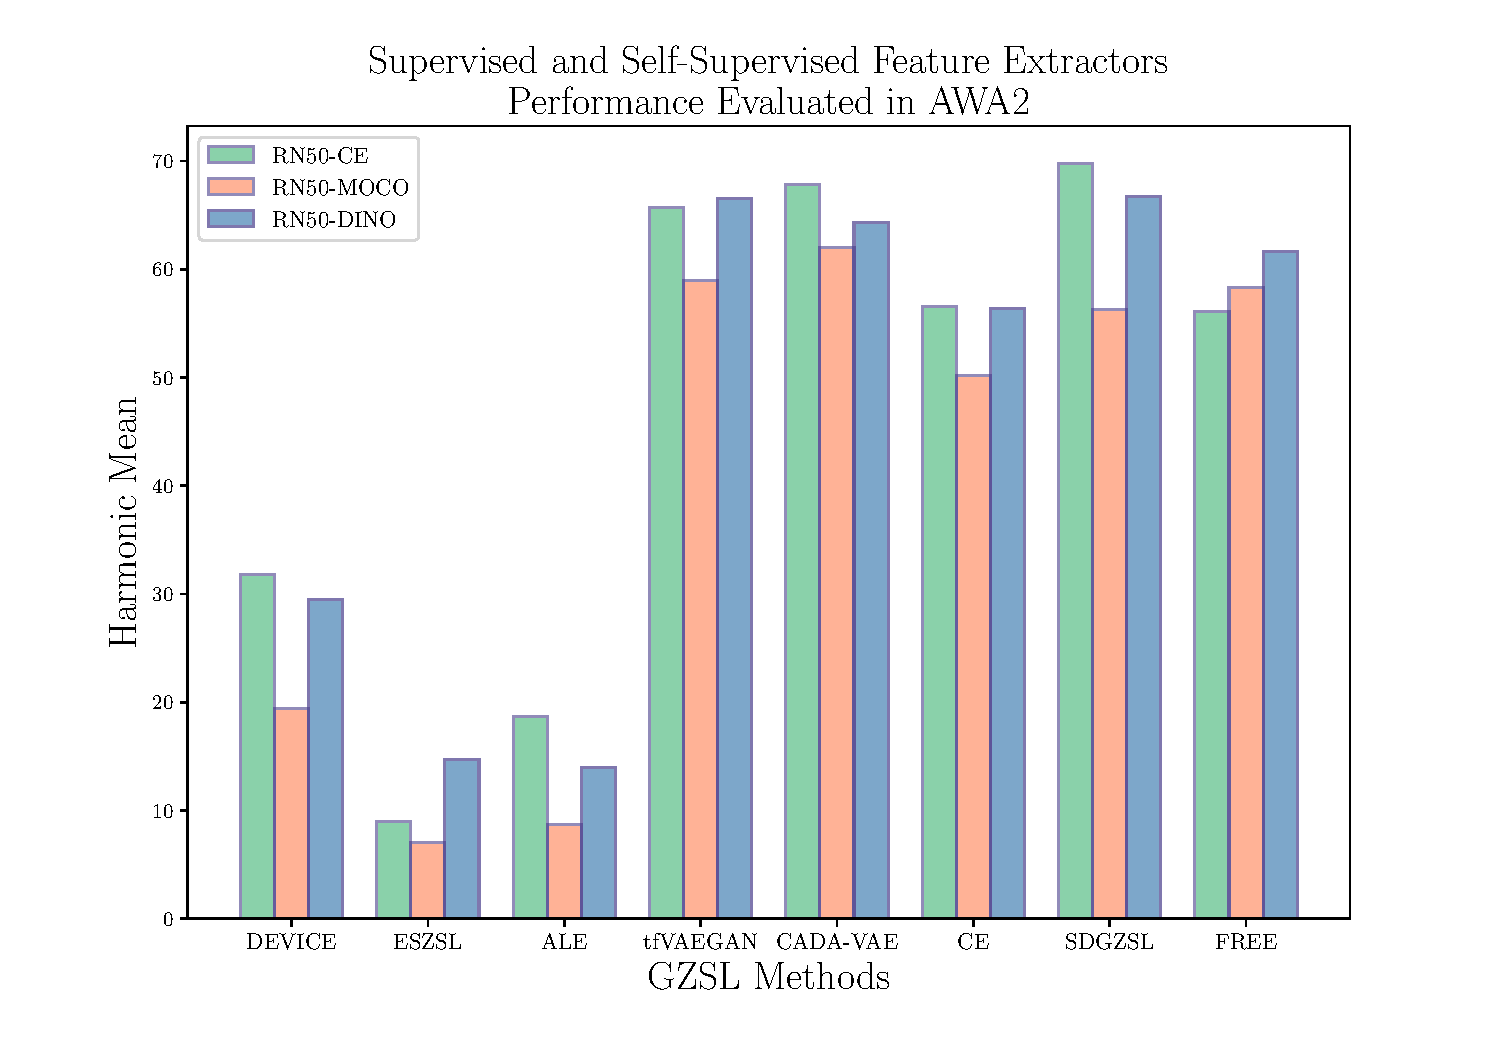
\includegraphics[align=t,width=\linewidth]{Images/awa2_diff_objs.pdf}
\end{minipage}%
 % \vspace{-0.05in}
 \caption{\textbf{Same Feature Extractor Pretrained with Different Learning Objectives.} We show the Harmonic Mean performance of different GZSL methods when using a RN50 model to extract the features of image samples from all datasets. RN50-\underline{CE} indicates that the model was pretrained using categorical cross-entropy in a supervised way, otherwise it was a model pretrained in a self-supervised way using a contrastive loss (RN50-\underline{MOCO}~\cite{MoCo} and RN50-\underline{DINO}~\cite{DINO}). All these models were pretrained using ImageNet-1k. Best viewed in color.}
 \label{fig:model_backbone_diff_objectives}
\end{figure*}